\chapter{Literature review and market research}\label{chap:lit}

\section{Environmental Requirements for Optimal Plant Growth }

Different plant species require a careful balance of light, temperature, humidity, and water supply to achieve optimal growth. The following sections outline the key environmental parameters that must be monitored and controlled to create ideal growing conditions within the greenhouse.

\subsection{Temperature} 

Plants regulate transpiration and cooling through specialized organs known as stomata located on the surface of leaves. These pores can open or close to control the release of water vapor, helping the plant manage water loss and internal temperature \cite{xu2024_high_temp_stomatal}. As ambient temperatures rise, open stomata allow for increased evaporation, aiding in the cooling process. However, excessive heat can lead to excessive water loss and stress. While optimal temperature ranges vary depending on the plant species and its growth stage, greenhouse temperatures are generally best maintained between \SI{15}{\degreeCelsius} and \SI{30}{\degreeCelsius} to support healthy plant development \cite{kosan2020}.

\subsection{Light} 

Light indirectly influences water loss in plants by triggering the opening of stomata, which enables gas exchange and \ce{CO2} uptake for photosynthesis \cite{kochetova2022}. However, excess light can cause overheating and increased transpiration, so it must be carefully managed along with temperature. Some plants are sensitive to photoperiodism, meaning their flowering depends on day length. In greenhouses, adjusting light exposure can control flowering times, allowing for year-round yield \cite{greenhouse_lighting}.

To evaluate light conditions within greenhouses, specific terminology and measurement units are used to describe both the quantity and quality of light that plants receive. The spectrum of light between 400 and 700~nanometres (nm) is recognized as \textbf{photosynthetically active radiation (PAR)}, the range most efficiently used by plants for photosynthesis \citep{sena2024}. Monitoring this specific light range is essential for optimizing plant productivity.

A key metric within the PAR range is the \textbf{photosynthetic photon flux density (PPFD)}. PPFD refers to the number of photons, within the PAR spectrum, that strike a square meter of plant surface each second. It is expressed in micromoles per square meter per second (\si{\micro\mole\per\metre\squared\per\second}). PPFD measurements help determine if the lighting levels in the greenhouse are sufficient to support healthy plant growth. Insufficient PPFD may lead to slow growth or poor productivity due to inadequate light. Excessively high PPFD can result in photoinhibition or physical damage to plant tissues \citep{measuring_ppfd}.

To relate PPFD to the more commonly used unit of \textit{lux}, an approximate conversion can be applied 
The exact factor depends on the spectrum of the light source, but for white LEDs, a typical approximation is:  

\begin{equation}
	\text{PPFD} \; (\si{\micro\mole\per\metre\squared\per\second}) 
	\;\approx\; \frac{\text{Illuminance (lux)}}{54} \label{ppfd}
\end{equation}

where 1~\si{\micro\mole\per\metre\squared\per\second} corresponds to roughly 54~lux. 
This relationship allows lux sensor readings to be interpreted in terms of usable light for photosynthesis.  \citep{ahn2017} Ideal PPFD ranges for Seedlings range from 100–300, while vegatative range from 300–600 \si{\micro\mole\per\metre\squared\per\second} \citep{definitiveGrowLight2024}. Monitoring and balancing light intensity through artificial lighting systems and proper greenhouse design is therefore essential to maintain optimal photosynthetic activity without causing plant stress.


\subsection{Humidity} 

Humidity plays a critical role in plant health by influencing the rate of transpiration, the process through which plants absorb water and nutrients from the soil and release water vapor through stomata. In high humidity environments, the air becomes too saturated with moisture, which suppresses transpiration. This reduction in water and nutrient uptake can hinder plant growth and development.

Conversely, in low humidity conditions, transpiration rates can become excessively high due to the dry air. In response, plants often close their stomata to conserve water, but this also limits gas exchange and light absorption, leading to water stress and reduced growth \cite{nederhoff}.

To support optimal development, research indicates that the ideal relative humidity (RH) range for most greenhouse crops lies between 30\% and 90\%. Maintaining this balance helps prevent both under- and over-transpiration, ensuring steady nutrient uptake and healthy physiological function \cite{pepper_guide}.



\subsection{Carbon Dioxide} 

For most greenhouse crops, net photosynthesis increases significantly as \ce{CO2} concentrations rise from ambient levels (approximately 340~ppm) up to around 1,000~ppm, potentially boosting photosynthesis by up to 50\%. However, the benefit of \ce{CO2} supplementation varies by crop and may not be economically justifiable under low light conditions or for certain species like tulips and Easter lilies, which show little response \cite{carbon_dioxide_enrichment}.

\ce{CO2} enters plants through stomata via diffusion, and its uptake is influenced by external \ce{CO2} concentration as well as factors such as light, temperature, humidity, and water availability. While plants generally grow well at ambient \ce{CO2} levels, concentrations can drop to as low as 200~ppm in sealed greenhouses during the day due to plant uptake. This drop can significantly reduce photosynthesis, sometimes with an effect comparable to the enhancement achieved by raising \ce{CO2} levels to 1,300~ppm.


\begin{figure}[h]
	\centering
	\fbox{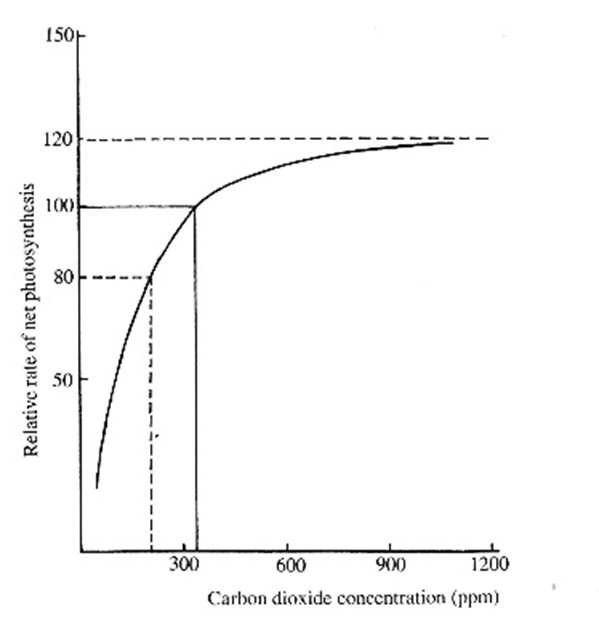
\includegraphics[width=0.55\textwidth]{figs/Co2.jpg}}
	\caption{Effect of \ce{CO2} concentration on photosynthesis rate. \cite{carbon_dioxide_enrichment}. }
	\label{fig:photosynthesis}
\end{figure}

As seen in the figure \ref{fig:photosynthesis}, at low \ce{CO2} concentrations (below approximately 300~ppm), the rate of photosynthesis increases sharply as \ce{CO2} concentration rises. However, beyond approximately 400--500~ppm (close to ambient fresh air levels), further increases in \ce{CO2} concentration have little to no additional effect on the photosynthesis rate, as the curve begins to plateau. Therefore, monitoring and maintaining ambient \ce{CO2} concentrations through simple ventilation can be sufficient to support healthy plant growth, without the need for costly \ce{CO2} enrichment.

\subsection{Water} 

A continuous supply of high-quality water is essential for plant transpiration, a process that not only cools the leaves but also facilitates the transport of nutrients from the roots to the leaves and fruits \cite{olabisi2022}.

To monitor soil moisture effectively, \textbf{Volumetric Water Content (VWC)} is commonly used. VWC is expressed as a percentage and represents the volume of water present in a given volume of soil.

\begin{equation}
\text{VWC (\%)} = \frac{\text{Volume of Water}~(\mathrm{cm}^3)}{\text{Volume of Soil}~(\mathrm{cm}^3)} \times 100
\end{equation}

This measurable metric provides valuable information for irrigation management, ensuring that plants receive adequate moisture for optimal growth without the risk of overwatering or water stress.


\section{Structural Design Standards}

\subsection{Achitecture of a greenhouse}\label{architecture}

Beyond structural integrity, the architectural design of the greenhouse plays a key role in regulating its internal climate. Greenhouses function either to retain heat during cold periods or to exclude heat in hotter seasons, with the aim of maintaining a productive microclimate for plant growth \cite{ghani2019}. In South Africa’s hot summers, a primary design consideration is minimizing heat buildup, making passive and active cooling essential.

One of the most influential architectural elements is the shape of the greenhouse, particularly the roof profile. The geometry directly affects solar irradiance levels inside the structure. In hot, arid environments, the optimal greenhouse form is one that minimizes solar gain during summer while maximizing it in winter, thereby supporting year-round cultivation. Research has shown that the roof angle and shape significantly influence the amount and distribution of solar radiation received \cite{ghani2019}.

A well-designed greenhouse structure must therefore strike a balance between mechanical resilience (to environmental loads) and thermal efficiency (to manage light and heat), with the shape and orientation of the building serving both functions. There are generally 4 main shapes discussed:

\begin{figure}[h]
    \centering
    \fbox{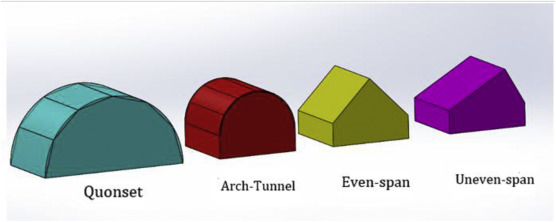
\includegraphics[width=0.8\textwidth]{figs/shapes.jpg}}
    \caption{Main Greenhouse Shapes. \cite{Sethi2009}. }
    \label{fig:photosynthesis}
\end{figure}

Choosing the right shape involves balancing structural load requirements with climate control goals, and often depends on regional weather patterns, crop types, and energy availability.

In terms of geographic suitability, greenhouse performance varies significantly with latitude and shape. For example, at \SI{31}{\degree}N latitude, even-span and Quonset greenhouses tend to receive more solar radiation in winter and less in summer, which is ideal for regions with significant seasonal temperature variation. However, at higher latitudes such as \SI{50}{\degree}N, uneven-span greenhouses are more effective for maintaining suitable internal conditions throughout the year.
\citep{Sethi2009}

The inclination angle significantly affects solar heat gain by altering the amount of radiation absorbed by the greenhouse surface. \citep{Mellalou2022}. As shown in figure \ref{fig:inclin} below, solar energy gaining rates decrease with steeper roof angles such as the \SI{27}{\degree} inclination angle seen below. While both N--S and E--W orientations perform similarly at \SI{12}{\degree} inclination, the E--W orientation consistently captures more energy at higher inclinations. This highlights the importance of optimizing both greenhouse orientation and tilt to balance heat gain and internal climate control.

\begin{figure}[h]
    \centering
    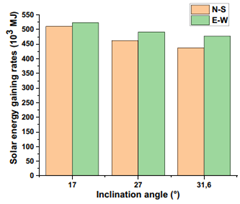
\includegraphics[width=0.95\textwidth]{figs/inclination.png}
    \caption{Solar radiation gain vs inclination angles \citep{Mellalou2022}. }
    \label{fig:inclin}
\end{figure}

\subsection{Sawtooth Design}

The sawtooth greenhouse has gained popularity in tropical and subtropical climates due to its unique roof design and natural ventilation system. This roof features several curved, sawtooth-shaped sections, with vertical windows at the highest points to enhance natural ventilation. It uses natural resources like airflow and gravity to regulate the temperature and humidity inside the greenhouse, reducing reliance on external energy sources such as electricity \citep{inson_greenhouse}. Compared to traditional greenhouses, sawtooth greenhouses provide better ventilation, temperature control, and structural stability, making them ideal for hot, humid regions. As the temperature inside the greenhouse rises, warm air naturally ascends and exits through the vertical windows at the top, while cooler air enters from below, creating a natural airflow cycle. The vertical windows are often controlled by a roll-up mechanism that opens for ventilation and closes for insulation when needed.

\begin{figure}[H]
    \centering
    \fbox{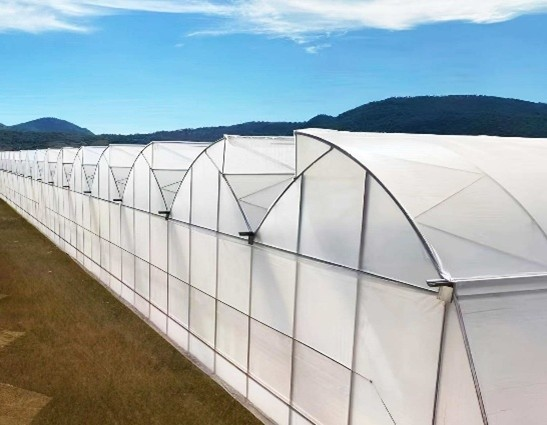
\includegraphics[width=0.45\textwidth]{figs/sawtooth.jpg}}
    \caption{Sawtooth Greenhouses \citep{inson_greenhouse}. }
    \label{fig:photosynthesis}
\end{figure}

\subsection{Construction techniques}

Greenhouses are classified by structure (wooden-, pipe-, and truss-framed) and by framing material. Wooden frames suit small, simple builds; pipe/steel frames add strength for larger spans; and truss systems deliver maximum rigidity for big installations. Materials are chosen for cost, durability, and maintenance: wood is cheap and accessible, however aluminium offers the best mix of strength, corrosion resistance, and low upkeep thus often the long-term choice \citep{dalai2020}.

\subsection{Covering materials}\label{cover}

The choice of covering material greatly influences the internal environment, light transmission, durability, and cost of a greenhouse. The most used materials include glass, plastic film, and rigid panels.

\textbf{Glass Greenhouses:} Glass offers high light transmission, good air circulation, and lower internal humidity, which helps reduce disease incidence. However, they are more expensive to build and maintain compared to plastic-covered structures. They introduce additional maintenance challenges and potential issues due to glass's fragile nature.

\textbf{Plastic Film Greenhouses:} Covered with flexible materials such as polyethylene, polyvinyl chloride, or polyester, plastic film greenhouses are cost-effective and require less heating. Their main disadvantage is a shorter lifespan, even UV-stabilized films typically last no more than 4 years.

\textbf{Rigid Panel Greenhouses:} Made from polycarbonate, fiberglass-reinforced plastic, acrylic, or PVC rigid panels, these coverings offer better durability (up to 20 years) and more uniform light distribution. However, the panels are prone to collecting dust and algae, which reduces light transmission over time \citep{verma2022}.

\section{Enviromental control}

Automated control of environmental parameters such as irrigation, heating and cooling, humidity, and airflow reduces manual workload and contributes to improved plant health. The following sections outline key industry standards and practices for managing these environmental factors effectively.

\subsection{Irrigation Systems}\label{irrig}

The right water system is key to the success of any greenhouse system. As greenhouse plants have a limited soil buffer, precision irrigation systems are vital to ensure high-quality crops and yields \citep{vegtech_netafim}.
Some of the most used types of irrigation include:

\textbf{Drip Irrigation:} This system delivers water directly to the base of each plant through a network of tubes and emitters, ensuring precise watering and minimizing water waste. By keeping foliage dry, it reduces the risk of fungal diseases. Drip irrigation is highly efficient and can be automated for consistent application \citep{cedar_greenhouse}.

\textbf{Misting System:} Misting systems distribute fine water droplets from above to hydrate plants and maintain humidity within the greenhouse. It provides broad and uniform coverage suitable for various crops, particularly delicate seedlings and humidity-loving plants. While effective for moisture control, excessive use can wet plant foliage, potentially elevating the risk of disease. Proper management is essential to mitigate these concerns.

\textbf{Ebb and Flow Systems:} Also known as flood and drain systems, ebb and flow setups periodically flood the growing area with nutrient-rich water and then allow it to drain away. This cyclical process ensures that plant roots receive adequate moisture and nutrients while preventing waterlogging. Ebb and flow systems are commonly used in hydroponic greenhouse operations \citep{floraflex_irrigation}. However, these systems require complex hydraulic components and precise nutrient management, increasing system complexity and maintenance requirements.

\subsection{Heating and Cooling Systems} \label{heat}

Efficient greenhouse climate control uses \textbf{passive} and \textbf{active} methods \citep{vegtech_netafim}. Passive approaches rely on natural processes and strategic design, needing no external energy; active systems use mechanical/electrical equipment requiring external energy inputs. 

\subsubsection*{Passive Heating}
This approach leverages solar energy to naturally warm the greenhouse. By incorporating design elements such as proper orientation, insulation, and thermal mass (e.g., water barrels or rock walls), heat is absorbed during the day and released at night, maintaining a stable internal temperature \citep{kumari2007}.

\subsubsection*{Active Heating}
To compensate for temperature drops, especially during winter nights, various heating systems are utilized. Options include unit heaters such as electric fan heaters, gas heating systems, heat lamps, and solar heating systems. The choice of system depends on factors such as greenhouse size, crop requirements, and energy efficiency considerations.

\subsubsection*{Passive Cooling}
Natural ventilation is employed to facilitate air exchange between the interior and exterior, helping to dissipate excess heat. This can be achieved through operable vents in the roof and sidewalls, allowing warm air to escape and cooler air to enter \citep{faridi_cooling}.

\subsubsection*{Active Cooling}
In situations where passive cooling is insufficient, active methods like evaporative cooling are implemented. This technique involves using fans and wet pads to cool the air through water evaporation, effectively reducing internal temperatures even during hot periods \citep{verma_cooling}. Integrating both passive and active systems allows for a comprehensive approach to climate control in greenhouses, ensuring optimal growing conditions across varying external temperatures and weather conditions.

\subsection{Humidity Control}

A cost-effective way to achieve humidity control in a controlled environment involves a misting system that sprays mist over the entire crop, thereby increasing humidity~\citep{controlling_humidity}. It is essential to recognize that relative humidity is strongly influenced by temperature: warm air can hold more moisture than cooler air. As temperatures drop, the relative humidity increases, even if the actual amount of water vapor in the air remains constant. \citep{Lawrence2005RHdewpoint}

Traditional humidity control methods often involve a combination of heating and ventilation. When humidity exceeds the desired level, greenhouse vents and windows can be opened to expel warm, moist air and allow cooler, drier air to enter. While this effectively reduces humidity, it can also result in unwanted heat loss. As a result, additional heating may be required to maintain optimal growing temperatures. Achieving a balance between ventilation and heating is therefore essential for stable humidity and temperature regulation within the greenhouse environment~\citep{pepper_guide}.

\subsection{Airflow}

\subsubsection*{Airflow in Greenhouse Environments}

Effective airflow is crucial in greenhouse environments to maintain optimal growing conditions and prevent plant diseases. Proper air movement helps disperse microclimates, preventing localized areas of trapped moisture, and ensures uniform temperature and humidity levels throughout the greenhouse. This uniformity is vital for consistent plant growth and reducing the risk of fungal infections~\citep{pepper_guide}.

\subsubsection*{Airflow Components in Greenhouses}

\begin{itemize}
    \item \textbf{Roof Vents:} These allow hot air to escape from the top of the greenhouse, facilitating natural convection. As warm air rises and exits, cooler air is drawn in, aiding in temperature regulation.

    \item \textbf{Side Vents:} Positioned along the sides, these vents promote cross-ventilation by enabling fresh air to flow horizontally through the structure. This movement helps maintain consistent temperature and humidity levels.

    \item \textbf{Intake and Exhaust Fans:} Mechanical systems that actively move air in and out of the greenhouse. Intake fans draw in fresh, usually cooler air, while exhaust fans expel stale, humid air, preventing the buildup of moisture and heat~\citep{airflow_growersnetwork}.

    \item \textbf{Horizontal Airflow (HAF) Fans:} These fans circulate air horizontally within the greenhouse, ensuring even distribution of temperature and humidity. By moving air consistently, HAF fans help eliminate microclimates and reduce condensation on plant surfaces, thereby lowering the risk of disease~\citep{lopez2013}.
\end{itemize}

\begin{figure}[h]
    \centering
    \begin{subfigure}[b]{0.45\textwidth}
        \centering
        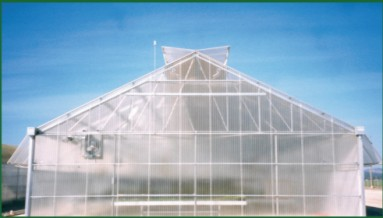
\includegraphics[width=\textwidth]{figs/airflow1.jpg}
        \caption{Greenhouse profile}
        \label{fig:image1}
    \end{subfigure}
    \hfill
    \begin{subfigure}[b]{0.45\textwidth}
        \centering
        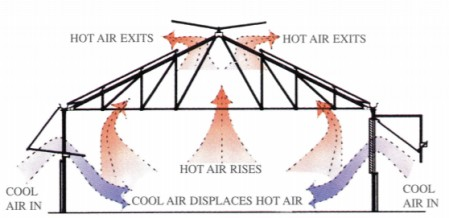
\includegraphics[width=\textwidth]{figs/airflow2.jpg}
        \caption{Ventilation airflow}
        \label{fig:image2}
    \end{subfigure}
    \caption{Airflow \citep{airflow_growersnetwork}}
    \label{fig:side_by_side}
\end{figure}

The figures above show an active ventilation system displaying the use of side and roof vents to promote healthy air circulation and thermal control. Integrating these components effectively creates a balanced airflow system that supports healthy plant development by regulating environmental conditions and minimizing disease-promoting factors.

\subsection{Automation and Environmental Control}

Automation in greenhouses allows for precise control of environmental conditions such as temperature, humidity, light, and \ce{CO2}. Using sensors and controllers, these systems enhance efficiency, minimize manual labor, and support consistent crop development. Depending on the greenhouse's complexity, control systems can range from simple microcontrollers to advanced PLCs and IoT-based architectures \citep{farooq2022}.

\subsubsection{Sensors}

\begin{itemize}
  \item \textbf{Temperature Sensors}: Monitor the internal temperature of the greenhouse.\\
  \textit{Common types}: Thermistors, RTDs, DS18B20 (digital)
  
  \item \textbf{Humidity Sensors}: Measure the ambient humidity levels.\\
  \textit{Common types}: DHT22, SHT31

  \item \textbf{Soil Moisture Sensors}: Detect the moisture content in soil.\\
  \textit{Common types}: Capacitive soil moisture sensors, resistive sensors

  \item \textbf{Light Sensors}: Measure light intensity reaching plant surfaces.\\
  \textit{Common types}: BH1750, TSL2561, TSL2591

  \item \textbf{\ce{CO2} Sensors}: Monitor carbon dioxide concentration.\\
  \textit{Common types}: MH-Z19, Senseair S8
\end{itemize}

Sensor data is fed into a controller, such as a PLC, Arduino, or Raspberry Pi, enabling automated decision-making for heating, cooling, irrigation, and other critical operations \citep{automated_greenhouse_iot}.


\subsubsection{Controllers} \label{control}

\textbf{Programmable Logic Controllers (PLC):} A Programmable Logic Controller (PLC) is a robust, industrial-grade computer used for controlling and monitoring industrial processes. It operates by receiving inputs, processing the data, and triggering outputs based on pre-programmed logic. PLCs are widely used in greenhouse automation due to their flexibility and reliability. Built with rugged designs and solid-state components, PLCs ensure long-term, reliable performance in harsh environments. The main drawback of PLCs is their higher power requirements and higher cost compared to microcontroller-based systems, which may limit their use in smaller or cost-sensitive projects \citep{dwinugroho2021greenhouse}.

\textbf{Microcontrollers:} Microcontrollers are small, programmable devices that can control a wide range of greenhouse automation tasks, such as environmental monitoring and data logging. The following microcontrollers are commonly used in greenhouse automation:

\begin{itemize}
    \item \textbf{Raspberry Pi:} A low-cost, powerful computer board frequently used in Internet of Things (IoT) applications. \citep{raspberrypi}. It offers greater processing power and versatility than simpler microcontrollers like Arduino and ESP8266. Raspberry Pi is ideal for more complex greenhouse automation systems, including advanced data collection and analysis 
    
    \item \textbf{ESP8266/ESP32:} These low-cost Wi-Fi microchips, developed by Espressif Systems, include built-in transmission control protocol (TCP/IP) stacks and microcontroller capabilities. The ESP8266 and ESP32 are widely used in IoT applications for connecting devices to the internet. They are compatible with the Arduino IDE, making them a popular choice for developing cost-effective, connected greenhouse systems \citep{esp_esp32}.
    
    \item \textbf{Arduino:} An open-source platform based on simple microcontroller chips, Arduino is designed for ease of use and flexibility. It is suitable for basic greenhouse monitoring and control tasks. Arduino's simplicity and large community make it an excellent choice for entry-level projects that require straightforward automation \citep{Yahaya2019}.
\end{itemize}

These controllers play a critical role in facilitating data logging and remote monitoring as well as enabling automated greenhouse systems to efficiently manage environmental factors such as temperature, humidity, and light for improved crop management.

\subsection{Wireless Connectivity and Actuation}

\textbf{Wireless Connection:}

ThingSpeak can be used with both Raspberry Pi and Arduino to wirelessly upload and visualize sensor data. ThingSpeak is an IoT analytics platform that allows real-time data collection, storage, and visualization from connected devices. Once connected to Wi-Fi, the Arduino or Raspberry Pi can send HTTP (Hypertext Transfer Protocol) requests to ThingSpeak's API (Application Programming Interface) to upload sensor readings. By integrating ThingSpeak with these controllers, one can effectively monitor and analyze sensor data remotely, making it a valuable tool for greenhouse automation and other IoT applications \citep{thingspeak}.

\textbf{Actuators and Switches:}

In greenhouse automation, relays are essential components that allow low-voltage control signals to switch high-voltage appliances such as irrigation pumps, lights, and ventilation systems on and off. This ensures efficient and safe operation of the system. These relays can be activated using the low voltage signals sent by the controller \citep{farooq2022}.

\section{Energy Efficiency \& Sustainability}

Solar power lets greenhouses run equipment on a clean, renewable source, cutting costs and environmental impact. Paired with batteries, it keeps systems running through outages and seasons, enabling stable, year-round crop production regardless of outside weather.

\subsection{Key Requirements for Solar System}

Incorporating a solar power system into a greenhouse requires understanding its essential components, each playing a pivotal role in energy capture, conversion, storage, and utilization. The key elements include:

\begin{enumerate}
    \item \textbf{Solar Panels (Photovoltaic Modules):} Solar panels are the primary components that capture sunlight and convert it into direct current (DC) electricity through photovoltaic cells \citep{Krisciunas2023}.
    
    \item \textbf{Inverter:} The inverter transforms the DC electricity generated by the solar panels into alternating current (AC) electricity
    
    \item \textbf{Charge Controller with Maximum Power Point Tracking (MPPT):} A charge controller manages the flow of electricity from the solar panels to the batteries, preventing overcharging and prolonging battery life. MPPT is an algorithm included in charge controllers used for extracting maximum available power from a PV module under varying conditions \citep{Eltawil2013}.
    
    \item \textbf{Batteries:} Batteries store electricity produced by the solar panels, providing energy during periods without sunlight or during power outages, ensuring continuous operation.
    
    \item \textbf{Mounting Systems:} Racking and mounting systems are crucial for securely installing solar panels on the greenhouse structure or the ground. This ensures that panels are positioned at an optimal angle to maximize solar exposure. Standard rails and brackets for various sizes exist on the market \citep{axe_struct_solar_mounting}.
\end{enumerate}

Understanding and integrating these components effectively is vital for the successful implementation of a solar-powered greenhouse, leading to enhanced energy efficiency and sustainability.
